% ]{beamer}
% \usepackage{handoutWithNotes}
% \pgfpagesuselayout{2 on 1 with notes}[letterpaper, landscape, border shrink=4mm]

\def\bmode{0} % Mode 0 for presentation, mode 1 for a handout with notes, mode 2 fo% r handout without notes
\if 0\bmode
\documentclass[smaller]{beamer}
\else \if 1\bmode
\immediate\write18{pdflatex -jobname=\jobname-Handout-Notes\space\jobname}
\documentclass[smaller,handout]{beamer}
\usepackage{handoutWithNotes}
\pgfpagesuselayout{2 on 1 with notes}[letterpaper, landscape, border shrink=4mm]
\else \if 2\bmode
\immediate\write18{pdflatex -jobname=\jobname-Handout\space\jobname}
\documentclass[smaller,handout]{beamer}
\fi
\fi
\fi

%%%%%%%%%%%%%%%%%%%%%%%%%%%%%%%%%%%%%%%%%%%%%%%%%%%%%%%%%%%%%%%%%%%%%%%%%%%%%%%%%%%%%%%%%%%%%
\newcommand{\coursetitle}{CEE 616: Probabilistic Machine Learning}
\newcommand{\longlecturetitle}{M2 Linear Methods: L2a Linear Discriminant Analysis}
\newcommand{\shortlecturetitle}{L2a: LDA}
\newcommand{\instructor}{Jimi Oke}
\newcommand{\lecturedate}{Tue, Sep 23, 2025}
%%%%%%%%%%%%%%%%%%%%%%%%%%%%%%%%%%%%%%%%%%%%%%%%%%%%%%%%%%%%%%%%%%%%%%%%%%%%%%%%%%%%%%%%%%%%%


% \usepackage[T1]{fontenc} 
% \usepackage{lmodern} 
%\usepackage{etex}
 %\newcommand{\num}{6{} }

% \usetheme[
%   outer/progressbar=foot,
%   outer/numbering=fraction,
%   block=fill,
%   inner/subsectionpage=progressbar
% ]{metropolis}
\usetheme{Madrid}
\useoutertheme[subsection=false]{miniframes} % Alternatively: miniframes, infolines, split
\useinnertheme{circles}
% %\useoutertheme{Frankfurt}
% \usecolortheme{beaver}
% %\useoutertheme{crane}
% %\useoutertheme{metropolis}
\usepackage[backend=biber,style=authoryear,maxcitenames=2,maxbibnames=99,safeinputenc,url=false, eprint=false]{biblatex}
%\addbibresource{bib/references.bib}
% \AtEveryCitekey{\iffootnote{{\tiny}\tiny}{\tiny}}

% %\usepackage{pgfpages}
% %\setbeameroption{hide notes} % Only slides
% %\setbeameroption{show only notes} % Only notes
% %\setbeameroption{hide notes} % Only notes
% %\setbeameroption{show notes on second screen=right} % Both

% % \usepackage[sfdefault]{Fira Sans}

% % \setsansfont[BoldFont={Fira Sans}]{Fira Sans Light}
% % \setmonofont{Fira Mono}

% %\usepackage{fira}
% %\setsansfont{Fira}
% %\setmonofont{Fira Mono}
% % To give a presentation with the Skim reader (http://skim-app.sourceforge.net) on OSX so
% % that you see the notes on your laptop and the slides on the projector, do the following:
% % 
% % 1. Generate just the presentation (hide notes) and save to slides.pdf
% % 2. Generate onlt the notes (show only nodes) and save to notes.pdf
% % 3. With Skim open both slides.pdf and notes.pdf
% % 4. Click on slides.pdf to bring it to front.
% % 5. In Skim, under "View -> Presentation Option -> Synhcronized Noted Document"
% %    select notes.pdf.
% % 6. Now as you move around in slides.pdf the notes.pdf file will follow you.
% % 7. Arrange windows so that notes.pdf is in full screen mode on your laptop
% %    and slides.pdf is in presentation mode on the projector.

% % Give a slight yellow tint to the notes page
% \setbeamertemplate{note page}{\pagecolor{yellow!5}\insertnote}\usepackage{palatino}

% %\usetheme{metropolis}
% %\usecolortheme{beaver}
 \usepackage{tipa}
% \usepackage{enumerate}
% \definecolor{darkcandyapplered}{HTML}{A40000}
% \definecolor{lightcandyapplered}{HTML}{e74c3c}

% %\setbeamercolor{title}{fg=darkcandyapplered}

% \definecolor{UBCblue}{rgb}{0.04706, 0.13725, 0.26667} % UBC Blue (primary)
% \definecolor{UBCgrey}{rgb}{0.3686, 0.5255, 0.6235} % UBC Grey (secondary)

% % \setbeamercolor{palette primary}{bg=darkcandyapplered,fg=white}
% % \setbeamercolor{palette secondary}{bg=darkcandyapplered,fg=white}
% % \setbeamercolor{palette tertiary}{bg=darkcandyapplered,fg=white}
% % \setbeamercolor{palette quaternary}{bg=darkcandyapplered,fg=white}
% % \setbeamercolor{structure}{fg=darkcandyapplered} % itemize, enumerate, etc
% % \setbeamercolor{section in toc}{fg=darkcandyapplered} % TOC sections
% % \setbeamercolor{frametitle}{fg=darkcandyapplered,bg=white} % TOC sections
% % \setbeamercolor{title in head/foot}{bg=white,fg=white} % TOC sections
% % \setbeamercolor{button}{fg=darkcandyapplered} % TOC sections

% % % Override palette coloring with secondary
% % \setbeamercolor{subsection in head/foot}{bg=lightcandyapplered,fg=white}

%\usecolortheme{crane}
% \makeatletter
% \setbeamertemplate{headline}{%
%   \begin{beamercolorbox}[colsep=1.5pt]{upper separation line head}
%   \end{beamercolorbox}
%   \begin{beamercolorbox}{section in head/foot}
%     \vskip1pt\insertsectionnavigationhorizontal{\paperwidth}{}{}\vskip1pt
%   \end{beamercolorbox}%
%   \ifbeamer@theme@subsection%
%     \begin{beamercolorbox}[colsep=1.5pt]{middle separation line head}
%     \end{beamercolorbox}
%     \begin{beamercolorbox}[ht=2.5ex,dp=1.125ex,%
%       leftskip=.3cm,rightskip=.3cm plus1fil]{subsection in head/foot}
%       \usebeamerfont{subsection in head/foot}\insertsubsectionhead
%     \end{beamercolorbox}%
%   \fi%
%   \begin{beamercolorbox}[colsep=1.5pt]{lower separation line head}
%   \end{beamercolorbox}
% }
% \makeatother

% Reduce size of frame box
\setbeamertemplate{frametitle}{%
    \nointerlineskip%
    \begin{beamercolorbox}[wd=\paperwidth,ht=2.0ex,dp=0.6ex]{frametitle}
        \hspace*{1ex}\insertframetitle%
    \end{beamercolorbox}%
}


%\setbeamercolor{frametitle}{bg=darkcandyapplered!80!black!90!white}
%\setbeamertemplate{frametitle}{\bf\insertframetitle}

%\setbeamercolor{footnote mark}{fg=darkcandyapplered}
%\setbeamercolor{footnote}{fg=darkcandyapplered!70}
%\Raggedbottom
%\setbeamerfont{page number in head/foot}{size=\tiny}
%\usepackage[tracking]{microtype}


% %\usepackage[sc,osf]{mathpazo}   % With old-style figures and real smallcaps.
% %\linespread{1.025}              % Palatino leads a little more leading

% % Euler for math and numbers
% %\usepackage[euler-digits,small]{eulervm}
% %\AtBeginDocument{\renewcommand{\hbar}{\hslash}}
\usepackage{graphicx,multirow,booktabs}
\usepackage{animate}
\usepackage{media9}


% %\mode<presentation> { \setbeamercovered{transparent} }

\setbeamertemplate{navigation symbols}{}
\makeatletter
\def\beamerorig@set@color{%
  \pdfliteral{\current@color}%
  \aftergroup\reset@color
}
\def\beamerorig@reset@color{\pdfliteral{\current@color}}
\makeatother


% %=== GRAPHICS PATH ===========
\graphicspath{{./m2-images/}}
% % Marginpar width
% %Marginpar width
% %\setlength{\marginparsep}{.02in}


% %% Captions
% % \usepackage{caption}
% % \captionsetup{
% %   labelsep=quad,
% %   justification=raggedright,
% %   labelfont=sc
% % }

% \setbeamerfont{caption}{size=\footnotesize}
% \setbeamercolor{caption name}{fg=darkcandyapplered}

% %AMS-TeX packages

\usepackage{amssymb,amsmath,amsthm,mathtools} 
\usepackage{bm}
\DeclareMathOperator*{\argmax}{arg\,max}
\DeclareMathOperator*{\argmin}{arg\,min}
% \usepackage{color}

% %https://tex.stackexchange.com/a/31370/2269
\usepackage{mathtools,cancel}

\renewcommand{\CancelColor}{\color{red}} %change cancel color to red

\makeatletter
\let\my@cancelto\cancelto %copy over the original cancelto command
\newcommand<>{\cancelto}[2]{\alt#3{\my@cancelto{#1}{#2}}{\mathrlap{#2}\phantom{\my@cancelto{#1}{#2}}}}
% redefine the cancelto command, using \phantom to assure that the
% result doesn't wiggle up and down with and without the arrow
\makeatother


% %\usepackage{comment}
% %\usepackage{hyperref,enumerate}
% \usepackage{minitoc,array}

% \definecolor{slblue}{rgb}{0,.3,.62}
% % \hypersetup{
% %     colorlinks,%
% %     citecolor=blue,%
% %     filecolor=blue,%
% %     linkcolor=blue,
% %     urlcolor=slblue
% % }

% \usepackage{epstopdf}
% \epstopdfDeclareGraphicsRule{.gif}{png}{.png}{convert gif:#1 png:\OutputFile}
% \AppendGraphicsExtensions{.gif}

% %\usepackage{listings}

% %%% TIKZ
% \usepackage{forest}
\usepackage{tikz}
\usepackage{pgfplots}
\usepackage{pgfplotstable}
%\usepackage{pgfgantt}
\pgfplotsset{compat=newest}

\usetikzlibrary{fit,arrows,shapes,positioning,shapes.geometric}
\usetikzlibrary{decorations.markings}
\usetikzlibrary{shadows,automata}
\usetikzlibrary{patterns}
\usetikzlibrary{trees,mindmap,backgrounds}
%\usetikzlibrary{circuits.ee.IEC}
\usetikzlibrary{decorations.text}
% % For Sagnac Picture
% \usetikzlibrary{%
%     decorations.pathreplacing,%
%     decorations.pathmorphing%
% }
% \tikzset{no shadows/.style={general shadow/.style=}}
% %
% %\usepackage{paralist}

% \tikzset{
%   font=\Large\sffamily\bfseries,
%   red arrow/.style={
%     midway,red,sloped,fill, minimum height=3cm, single arrow, single arrow head extend=.5cm, single arrow head indent=.25cm,xscale=0.3,yscale=0.15,
%     allow upside down
%   },
%   black arrow/.style 2 args={-stealth, shorten >=#1, shorten <=#2},
%   black arrow/.default={1mm}{1mm},
%   tree box/.style={draw, rounded corners, inner sep=1em},
%   node box/.style={white, draw=black, text=black, rectangle, rounded corners},
% }

% %%% FORMAT PYTHON CODE
% %\usepackage{listings}
% % Default fixed font does not support bold face
% \DeclareFixedFont{\ttb}{T1}{txtt}{bx}{n}{8} % for bold
% \DeclareFixedFont{\ttm}{T1}{txtt}{m}{n}{8}  % for normal

% % Custom colors
% \definecolor{deepblue}{rgb}{0,0,0.5}
% \definecolor{deepred}{rgb}{0.6,0,0}
% \definecolor{deepgreen}{rgb}{0,0.5,0}

% %\usepackage{animate}

% % Python style for highlighting
% % \newcommand\pythonstyle{\lstset{
% % language=Python,
% % basicstyle=\footnotesize\ttm,
% % otherkeywords={self},             % Add keywords here
% % keywordstyle=\footnotesize\ttb\color{deepblue},
% % emph={MyClass,__init__},          % Custom highlighting
% % emphstyle=\footnotesize\ttb\color{deepred},    % Custom highlighting style
% % stringstyle=\color{deepgreen},
% % frame=tb,                         % Any extra options here
%     % showstringspaces=false            % 
% % }}

% % % Python environment
% % \lstnewenvironment{python}[1][]
% % {
% % \pythonstyle
% % \lstset{#1}
% % }
% % {}

% % % Python for external files
% % \newcommand\pythonexternal[2][]{{
% % \pythonstyle
% % \lstinputlisting[#1]{#2}}}

% % Python for inline
% % 
% % \newcommand\pythoninline[1]{{\pythonstyle\lstinline!#1!}}

% %\usepackage{algorithm2e}

\newcommand{\eps}{\epsilon}
\newcommand{\bX}{\mb X}
\newcommand{\by}{\mb y}
\newcommand{\bbe}{\bm\beta}
\newcommand{\beps}{\bm\epsilon}
\newcommand{\bY}{\mb Y}

\newcommand{\osn}{\oldstylenums}
\newcommand{\dg}{^{\circ}}
\newcommand{\lt}{\left}
\newcommand{\rt}{\right}
\newcommand{\pt}{\phantom}
\newcommand{\tf}{\therefore}
\newcommand{\?}{\stackrel{?}{=}}
\newcommand{\fr}{\frac}
\newcommand{\dfr}{\dfrac}
\newcommand{\ul}{\underline}
\newcommand{\tn}{\tabularnewline}
\newcommand{\nl}{\newline}
\newcommand\relph[1]{\mathrel{\phantom{#1}}}
\newcommand{\cm}{\checkmark}
\newcommand{\ol}{\overline}
\newcommand{\rd}{\color{red}}
\newcommand{\bl}{\color{blue}}
\newcommand{\pl}{\color{purple}}
\newcommand{\og}{\color{orange!90!black}}
\newcommand{\gr}{\color{green!40!black}}
\newcommand{\dca}{\color{darkcandyapplered}}
\newcommand{\nin}{\noindent}
\newcommand*\circled[1]{\tikz[baseline=(char.base)]{
            \node[shape=circle,draw,thick,inner sep=1pt] (char) {\small #1};}}

\newcommand{\bc}{\begin{compactenum}[\quad--]}
\newcommand{\ec}{\end{compactenum}}

\newcommand{\p}{\partial}
\newcommand{\pd}[2]{\frac{\partial{#1}}{\partial{#2}}}
\newcommand{\dpd}[2]{\dfrac{\partial{#1}}{\partial{#2}}}
\newcommand{\pdd}[2]{\frac{\partial^2{#1}}{\partial{#2}^2}}
\newcommand{\pde}[3]{\frac{\partial^2{#1}}{\partial{#2}\partial{#3}}}
\newcommand{\nmfr}[3]{\Phi\left(\frac{{#1} - {#2}}{#3}\right)}
\newcommand{\Err}{\text{Err}}
\newcommand{\err}{\text{err}}

%\DeclarePairedDelimiter\ceil{\lceil}{\rceil}
%\DeclarePairedDelimiter\floor{\lfloor}{\rfloor}

%%%% GREEK LETTER SHORTCUTS %%%%%
\newcommand{\la}{\lambda}
\renewcommand{\th}{\theta}
\newcommand{\al}{\alpha}
\newcommand{\G}{\Gamma}
\newcommand{\si}{\sigma}
\newcommand{\Si}{\Sigma}


\pgfmathdeclarefunction{poiss}{1}{%
  \pgfmathparse{(#1^x)*exp(-#1)/(x!)}%
  }

\pgfmathdeclarefunction{gauss}{2}{%
  \pgfmathparse{1/(#2*sqrt(2*pi))*exp(-((x-#1)^2)/(2*#2^2))}%
}

\pgfmathdeclarefunction{expo}{2}{%
  \pgfmathparse{#1*exp(-#1*#2)}%
}

\pgfmathdeclarefunction{expocdf}{2}{%
  \pgfmathparse{1 -exp(-#1*#2)}%
}

\newcommand{\mb}{\mathbb}
\newcommand{\mc}{\mathcal}
\newcommand{\tr}{^{\top}}
\newcommand{\pe}{\pause}
% \usepackage{pst-plot}

% \usepackage{pstricks-add}
% \usepackage{auto-pst-pdf}   

% \psset{unit = 3}

% \def\target(#1,#2){%
%  {\psset{fillstyle = solid}
%   \rput(#1,#2){%
%     \pscircle[fillcolor = white](0.7,0.7){0.7}
%     \pscircle[fillcolor = blue!60](0.7,0.7){0.5}
%     \pscircle[fillcolor = white](0.7,0.7){0.3}
%     \pscircle[fillcolor = red!80](0.7,0.7){0.1}}}}
% \def\dots[#1](#2,#3){%
%     \psRandom[
%       dotsize = 2pt,
%       randomPoints = 25
%     ](!#2 #1 0.04 sub sub #3 #1 0.04 sub sub)%
%      (!#2 #1 0.04 sub add #3 #1 0.04 sub add)%
%      {\pscircle[linestyle = none](#2,#3){#1}}}


%%%%%%%%%%%%%%%%%%%%%%%%%%%%%%%%%%%%%%%%%%%%%%%%%%%
%%%%%%%%%%%%%%%%%%%%%%%%%%%%%%%%%%%%%%%%%%%%%%%%%%%
\title[\shortlecturetitle]{ {\normalsize \coursetitle}
  \\ \longlecturetitle}
\date[\lecturedate]{\footnotesize \lecturedate}
\author{{\bf \instructor}}
\institute[UMass Amherst]{
%\titlegraphic{\hfill
  \begin{tikzpicture}[baseline=(current bounding box.center)]
    \node[anchor=base] at (-7,0) (its) {
\includegraphics[scale=.3]{UMassEngineering_vert}} ;
  \end{tikzpicture}
  % \hfill\includegraphics[height=1.5cm]{logo}
}

%https://tex.stackexchange.com/questions/55806/mindmap-tikzpicture-in-beamer-reveal-step-by-step
  \tikzset{
    invisible/.style={opacity=0},
    visible on/.style={alt={#1{}{invisible}}},
    alt/.code args={<#1>#2#3}{%
      \alt<#1>{\pgfkeysalso{#2}}{\pgfkeysalso{#3}} % \pgfkeysalso doesn't change the path
    },
  }


% https://tex.stackexchange.com/questions/446468/labels-with-arrows-for-an-equation
% https://tex.stackexchange.com/a/402466/121799
\newcommand{\tikzmark}[3][]{
\ifmmode
\tikz[remember picture,baseline=(#2.base)] \node [inner sep=0pt,#1](#2) {$#3$};
\else
\tikz[remember picture,baseline=(#2.base)] \node [inner sep=0pt,#1](#2) {#3};
\fi
}

% \lstset{language=matlab,
%                 basicstyle=\scriptsize\ttfamily,
%                 keywordstyle=\color{blue}\ttfamily,
%                 stringstyle=\color{blue}\ttfamily,
%                 commentstyle=\color{gray}\ttfamily,
%                 morecomment=[l][\color{gray}]{\#}
%               }


              
\begin{document}

\maketitle

\begin{frame}
  \frametitle{Outline}
  \tableofcontents
\end{frame}

 


% \section{Recap: Logistic MLE \& Performance}

%  \begin{frame}
%    \frametitle{Summary}
%    \label{recap}
%   \begin{itemize}
%   \item The simple logistic regression model (binary case) is given by:
%       \begin{equation}
%       \label{eq:1}
%       p(X) = \fr{e^{\beta_0 + \beta_1X}}{1 + e^{\beta_0 + \beta_1X}}
%     \end{equation}
%   \item   The log-likelihood of a sample of $n$ observations in the binary response case is:
%     \begin{equation}
%      \ell(\bm\beta) = \sum_i \lt[ y_i\lt(\beta_0 + \beta_1x_i \rt) - \log\lt(1 + e^{\beta_0 + \beta_1x_i}\rt) \rt]
%    \end{equation}
%    \item Based on the principle of maximum likelihood, the estimate $\hat\beta$ is given by the maximizing value of $\ell$.

%    \item    This can be solved via gradient ascent or Newton-Raphson.

%    \item Logistic regression and simple linear regression are both specifications of the Generalized Linear Model \hyperlink{glm}{\beamerbutton{Appendix}}
%  \end{itemize}

%  \end{frame}

%  \begin{frame}
%    \frametitle{Summary (cont.)}
%    \textbf{Gradient ascent for logistic regression}
%    \begin{equation}
%      \beta_{k+1} = \beta_k + \lambda\nabla\ell(\beta_k)
%    \end{equation}

%    \textbf{Newton-Raphson method for logistic regression}
%    \begin{equation}
%       \beta_{k+1} = \beta_k - {\bm H}^{-1}_{\beta_k}(\ell)\nabla_{\beta_k}\ell(\beta_k)
%    \end{equation}
%   This can be rewritten as:
%   \begin{equation}
%     \beta_{k+1} = (\bm X^T \bm W \bm X)^{-1}\bm X^T \bm W \bm z
%   \end{equation}
%   where $\bm z = \bm X\beta_k + \bm W^{-1}(\bm y - \bm p)$.

%   \begin{itemize}
%   \item Also known as iteratively reweighted least squares (IRLS)
%  \end{itemize}

% \end{frame}

% \begin{frame}
%   \frametitle{Classification metrics}
  
%  \pause
%  \begin{itemize}\small
%  %\item Error rate\pause
%  \item \textbf{Accuracy} = 1 $-$ Error rate: \pause
%    \begin{equation}
%      Acc = \fr{TP + TN}{P + N} = \pause \fr{TP + TN}{TP + TN + FP + FN}
%    \end{equation}
%    \pause
   
%  \item \textbf{Sensitivity/Recall}:       (True positive rate/power/1 - Type II error) \pause
%    \begin{equation}
%      Re = \fr{TP}{P} \pause = \fr{TP}{TP + FN}
%    \end{equation}
%    \pause
%  \item \textbf{Precision} (positive prediction value): \pause
%    \begin{equation}
%      Pr = \fr{TP}{P^{*}} \pause  = \fr{TP}{TP + FP}
%    \end{equation}\pause
%  \item \textbf{Specificity} (True negative rate): \pause
%    \begin{equation}
%      TNR = \fr{TN}{N} \pause = \fr{TN}{TN + FP}
%    \end{equation} \pause
%  \item      False positive rate (Type I error/$1-$Specificity/fallout): \pause
%    \begin{equation}
%      FPR = \pause \fr{FP}{N} = \pause \fr{FP}{FP + TN} \pause = 1 - TNR
%    \end{equation}
%    \pause
%  %\item Others: false omission rate, false negative rate, etc
%  \end{itemize}

% \end{frame}

% \begin{frame}
%   \frametitle{Classification metrics (cont.)}
%   \pause

%   \begin{itemize}
%   \item $F_{1}$ score (harmonic mean of precision and recall): \pause
%     \begin{equation}
%       F_{1} = \fr{2}{\fr{1}{Re} + \fr{1}{Pr}} = \fr{TP}{TP + \fr12\lt(FP + FN\rt)}
%     \end{equation}

%   \item Area under receiver operating characteristics (ROC) curve (AUC): \pause
%     \begin{itemize}
%     \item The ROC curve plots TPR (recall) vs FPR (fallout) at various thresholds
%     \item A perfectly accurate model would have an AUC of 1.
%     \end{itemize}
%   \end{itemize}
% \end{frame}

 

 
\section{Introduction}
\begin{frame}
  \frametitle{Why classify?}
  Consider the following plot:\pause

  \begin{center}
    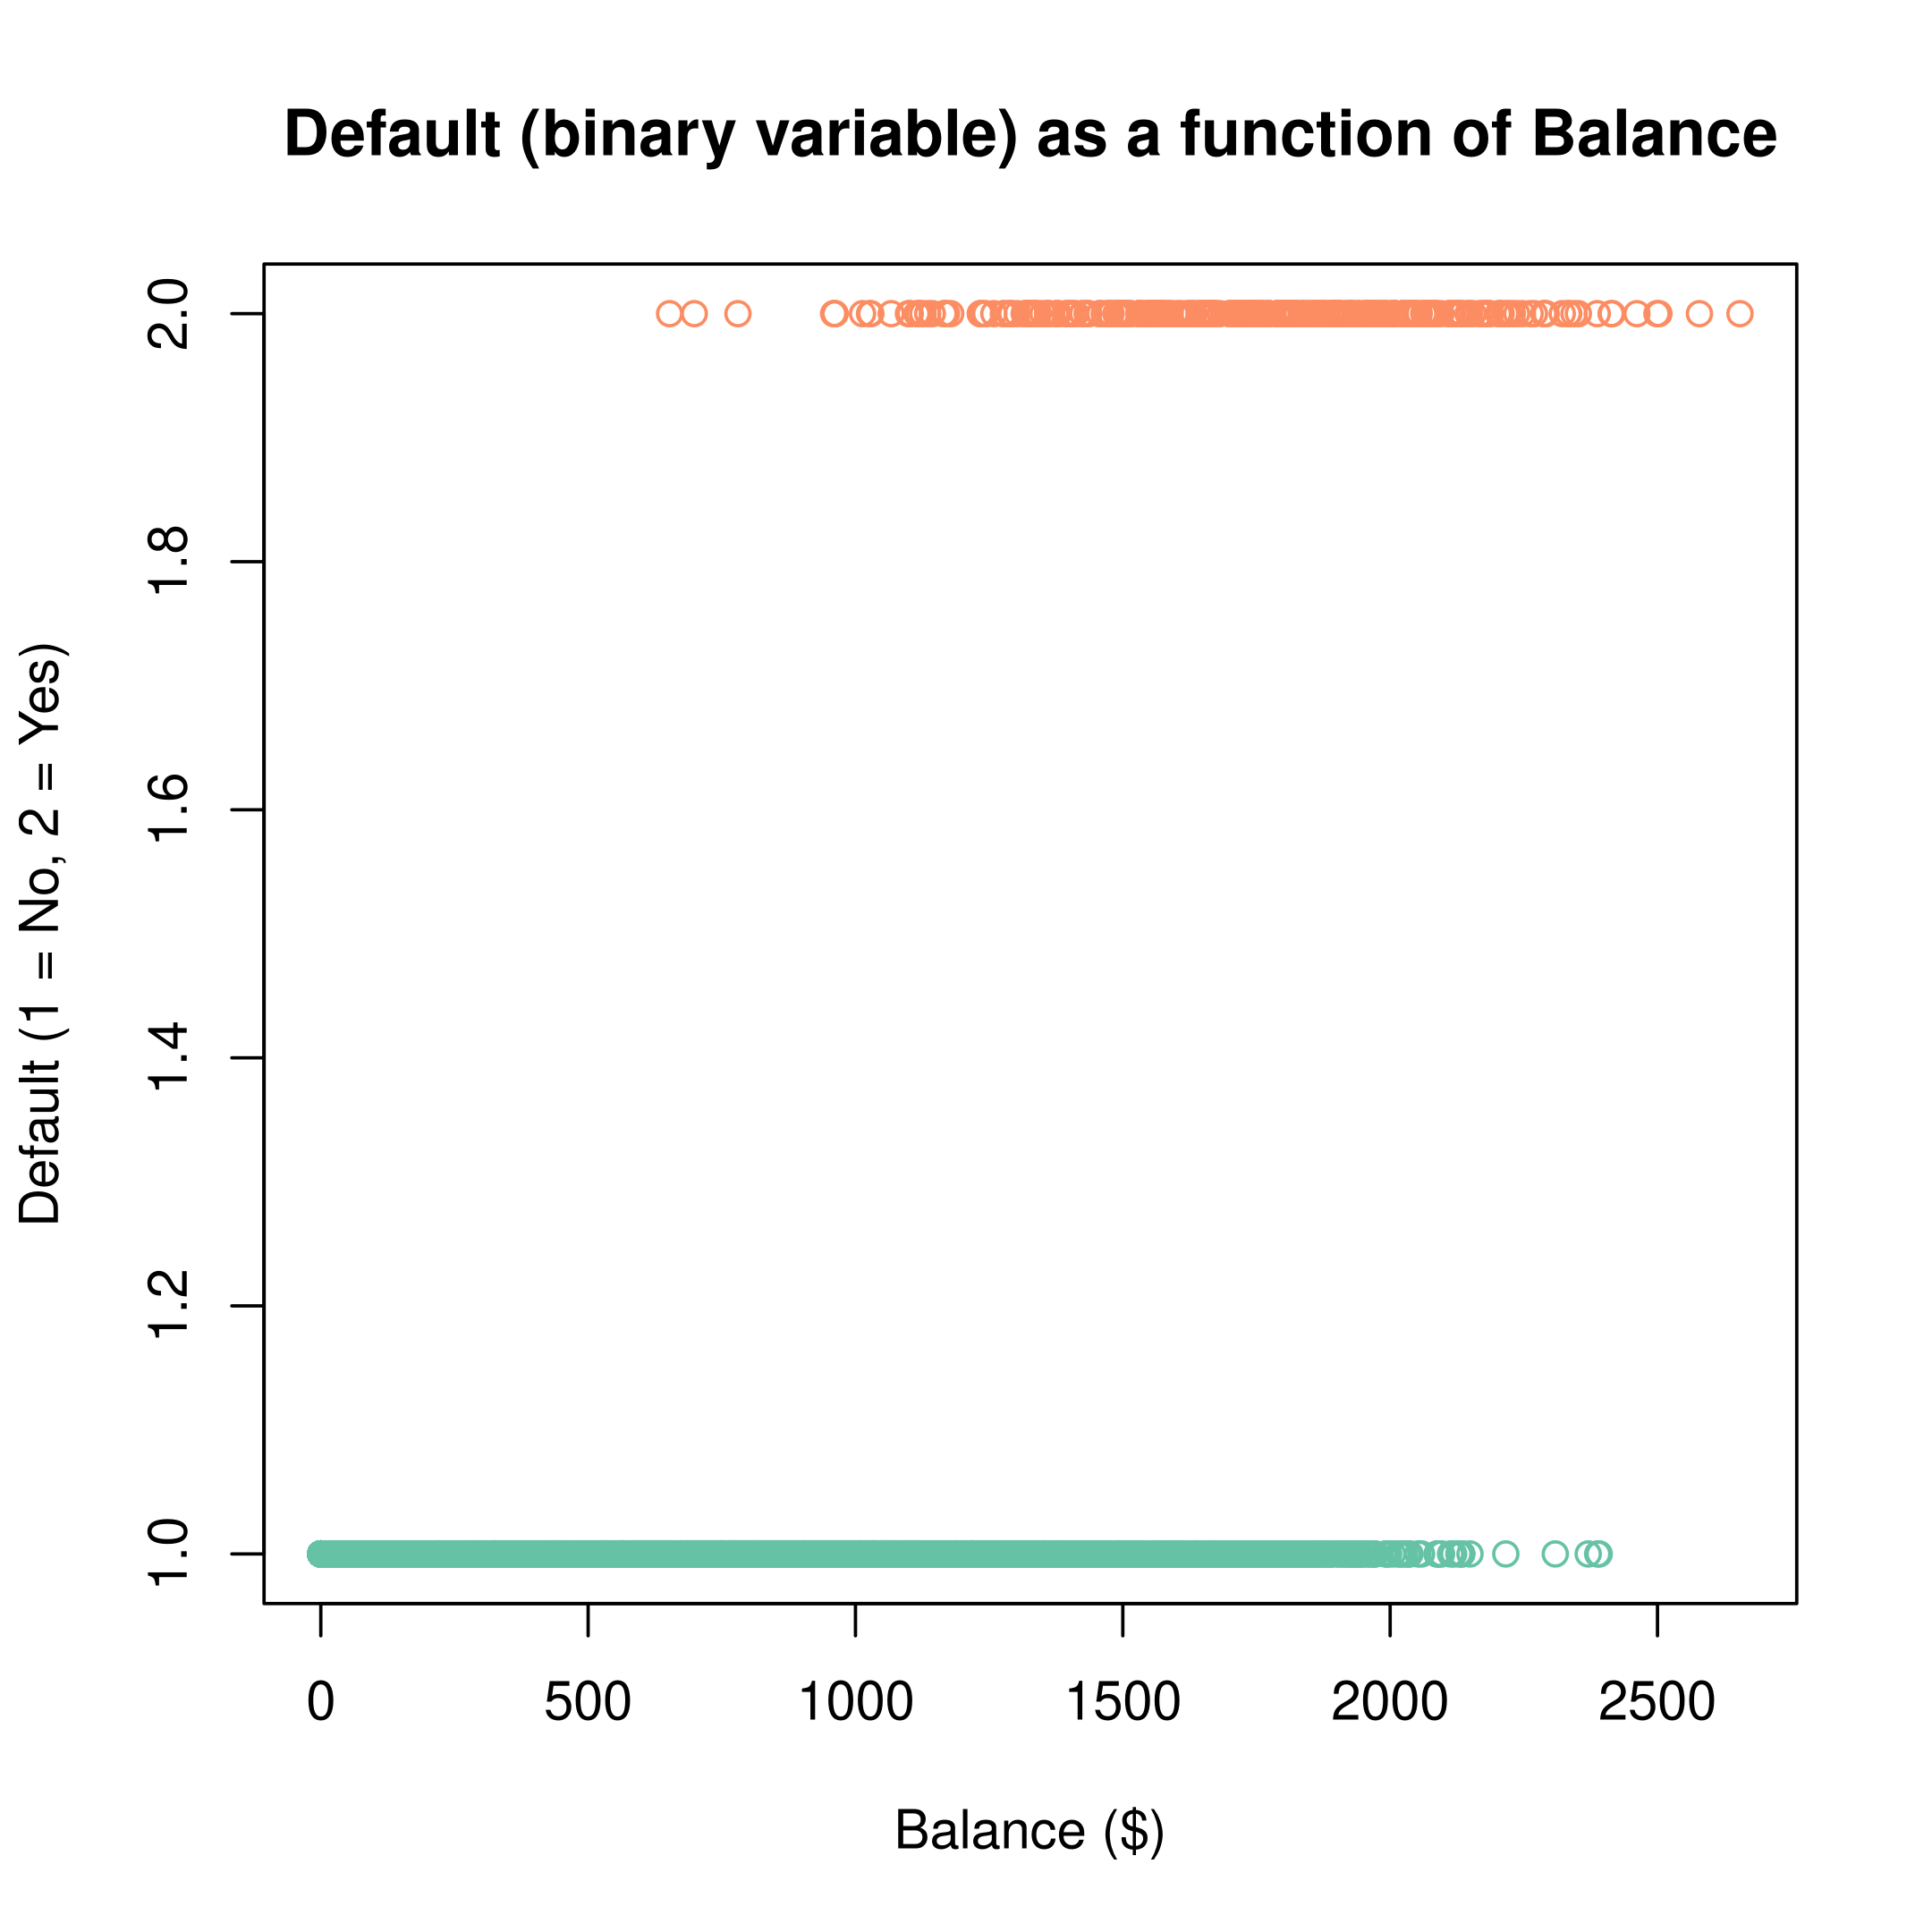
\includegraphics[width=.5\textwidth]{default-balance}
  \end{center}
  \pause
  What problems would we face if we tried to fit a linear model to these data?
\end{frame}

\begin{frame}
  \frametitle{The classification problem}
  \pause
  Consider the following plot
  \pause
  \begin{center}
    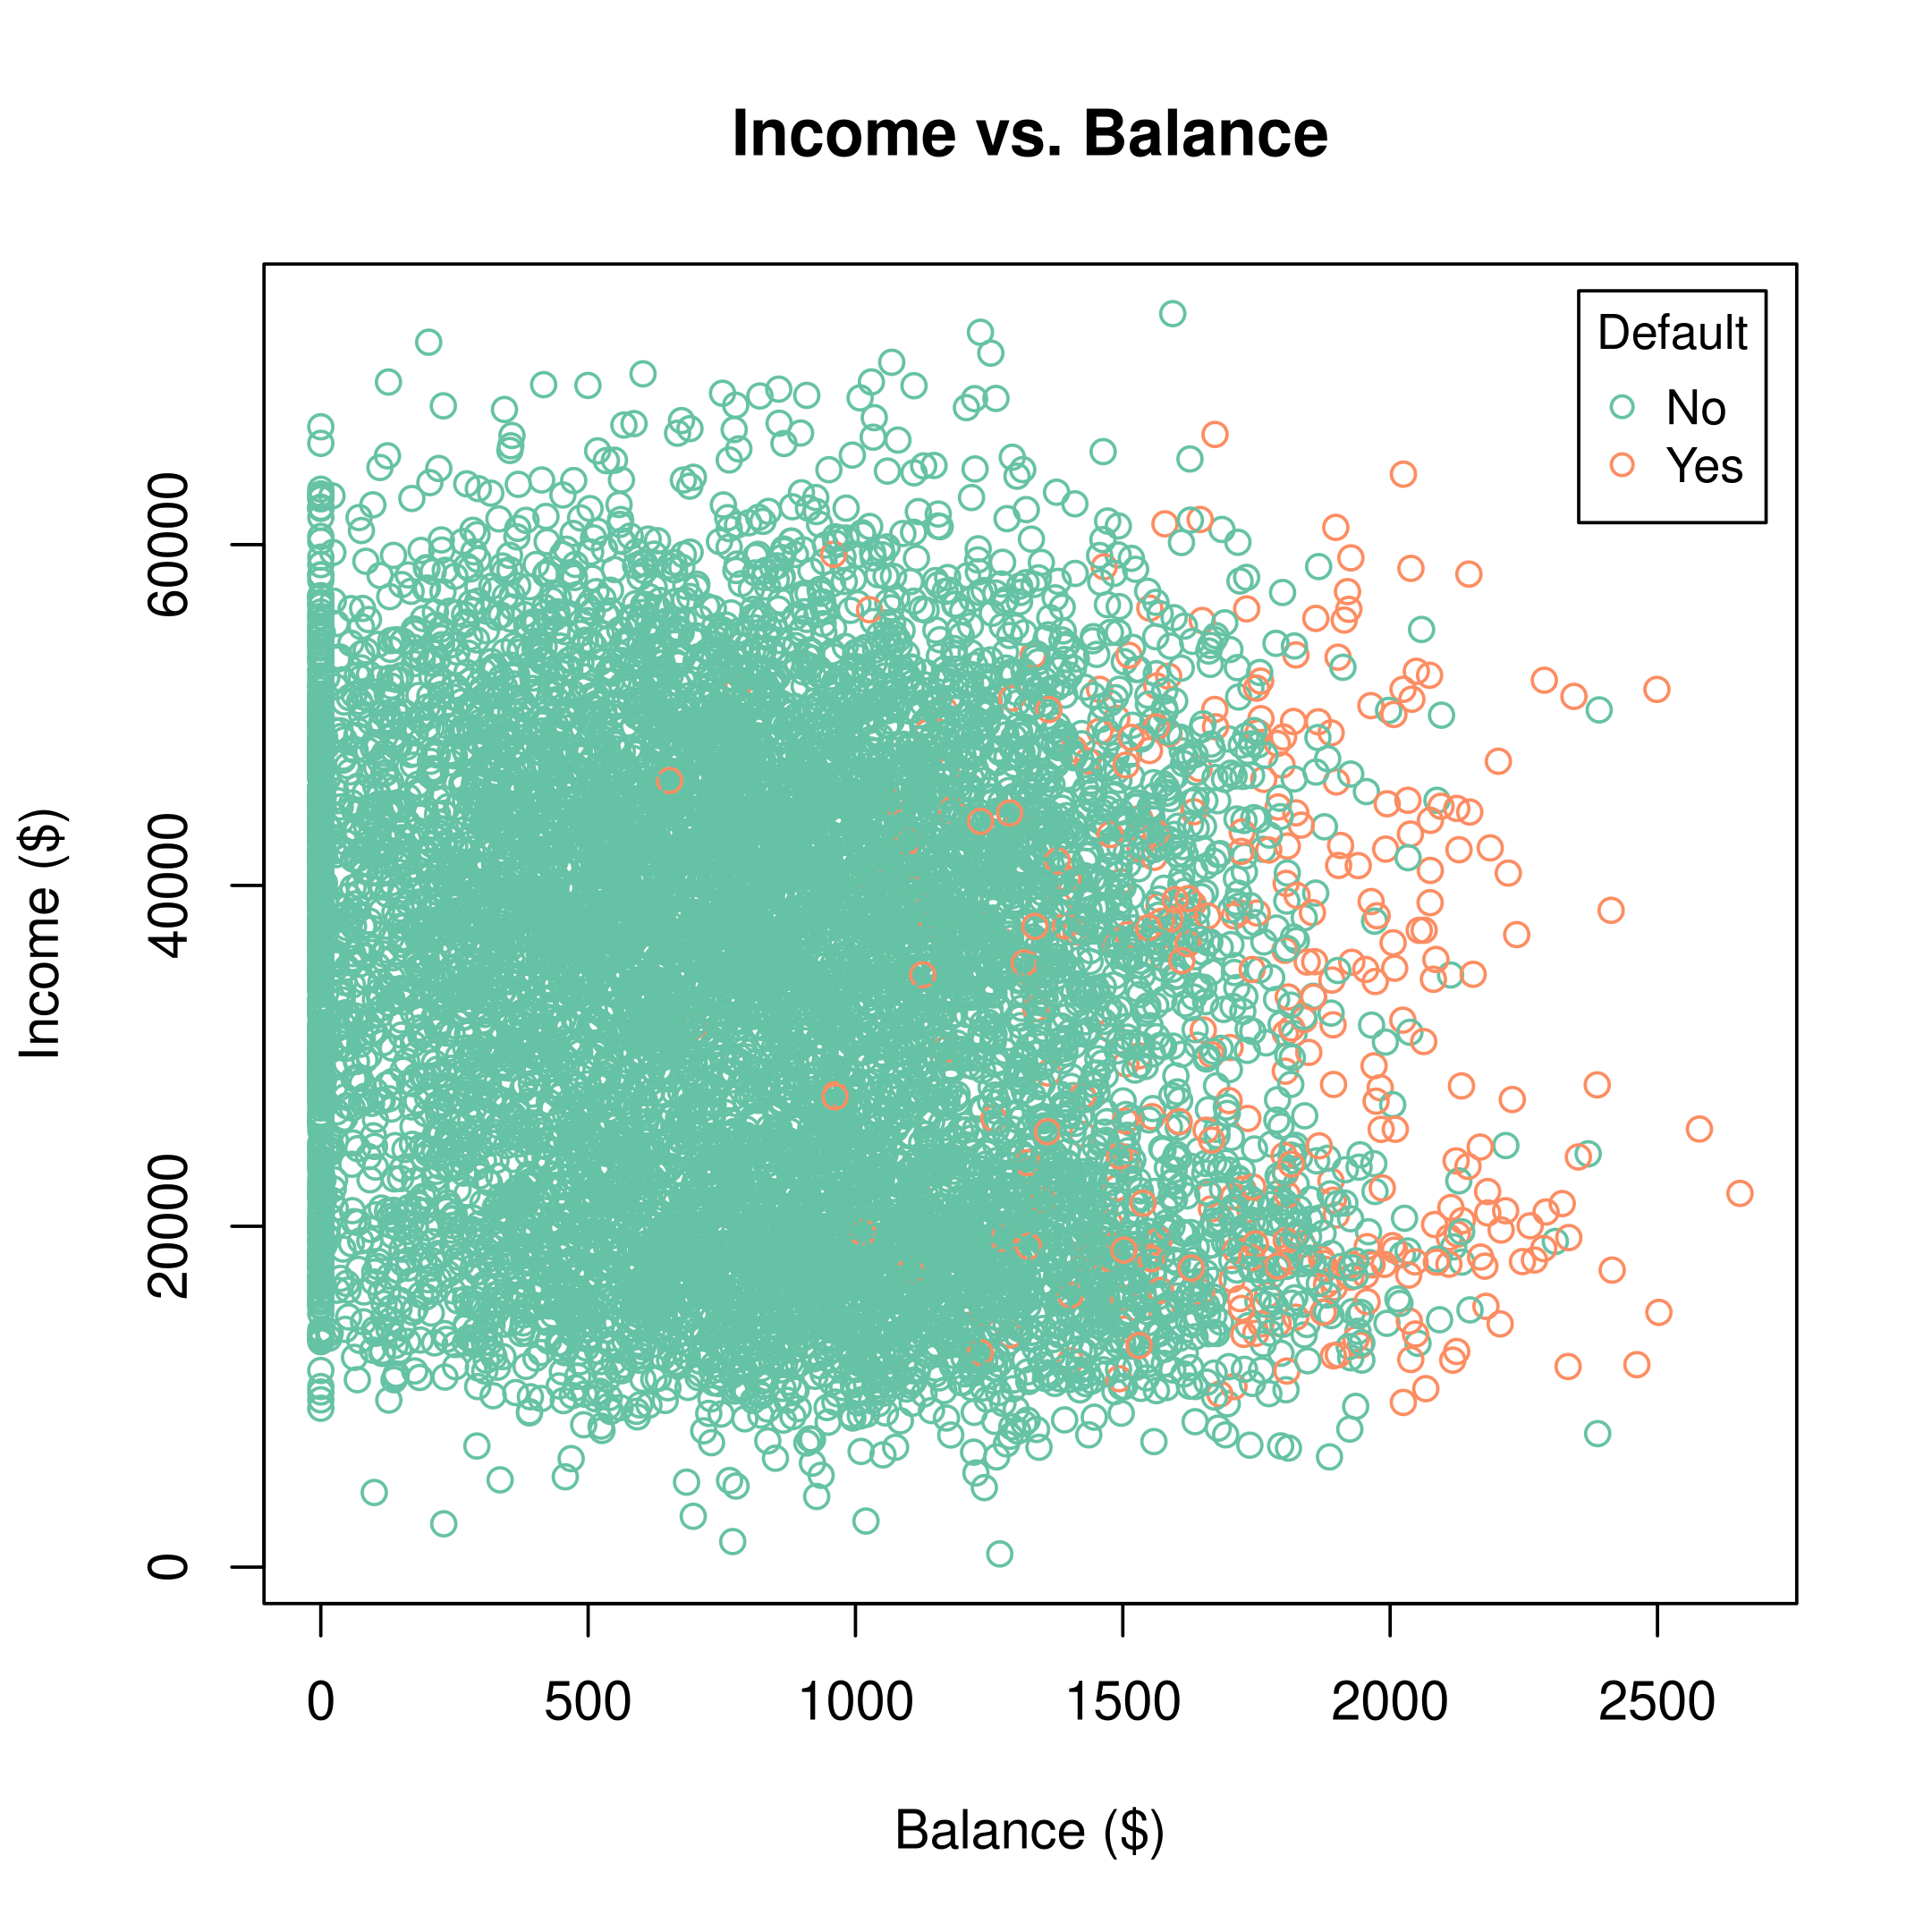
\includegraphics[width=.5\textwidth]{income-balance}
  \end{center}
  \pause
  How would you estimate a model to classify a point $(x_{(i,\mathtt{balance})},x_{(i,\mathtt{income})})$?
  \end{frame}
  


% \begin{frame}
%   \frametitle{Topics and objectives}
%   \pause

%   In this lecture and the next, we will cover the following methods:
%   \pause
  
%   \begin{itemize}[<+->]
%   \item Bayes Classifier and K Nearest Neighbors (KNN)
%   \item Logistic Regression
%   \item Linear discriminant analysis (LDA) \pause
%     \begin{itemize}[<+->]
%     \item And its variant: quadratic discriminant analysis (QDA)
%     \end{itemize}
%   \end{itemize}
%   \pause

%   Finally, we will:
% \pause
%   \begin{itemize}
%    \item Compare the performance of logistic regression, LDA, QDA and KNN
%   \end{itemize}
% \pause
%   \begin{block}{Module objectives}\pause
%     \begin{itemize}[<+->]
%     \item Understand the theoretical framework for basic classification methods: logistic/LDA/QDA/KNN\pause
%     \item Recognize classification problems in engineering and know how to efficiently apply these methods
%     \end{itemize}
%   \end{block}
% \end{frame}


  \begin{frame}
  \frametitle{Bayes theorem for classification}
  \pause
  Given: \pause
  \begin{itemize}
  \item The conditional density of a variable $\bm x$ in class $c$: \pause $p_{c}(\bm x)$ \pause
  \item The prior probability of class $c$: \pause $\pi_{c}$\pause
    \begin{equation}
     \text{such that: }\pause  \sum_{c=1}^{C} \pi_{c} = 1
    \end{equation}
  \end{itemize}

  \pause

  Then, using Bayes theorem, we write \textbf{class posterior} as: \pause
  \begin{equation}
    p(y = c| \bm x) \pause = \fr{p_{c}(\bm x)\pi_{c}}{\sum_{c'=1}^{C}p_{c'}(\bm x)\pi_{c'}}
  \end{equation}
  \pause
  With the class posteriors, we can then assign an observation $i$ using the Bayes' classifier:\pause
  \begin{equation}
    y^{*}_{i} = \arg\max_{k}p(y= c|\bm x_{i})
  \end{equation}
  \pause
  (i.e. we assign to the class with the maximum probability)
\end{frame}

\begin{frame}
  \frametitle{Generative classifiers}
  \pe
  A generative classifier is a model of the form:\pe
  \begin{equation}
    p(y=c|\bm x;\bm\th) = \fr{p(\bm x|y = c;\bm\th)p(y=c;\bm\th)}{\sum_{c'}p(\bm x|y = c';\bm\th)p(y=c;\bm\th)}
  \end{equation}
  \pe
  where:
  \begin{itemize}
  \item $p(y=c;\bm\th)$ is the class prior\pe
  \item $p( \bm x|y =c;\bm\th)$ is the class conditional density for class $c$\pe
  \item Generative classifiers generate features for each class by sampling from the class conditional density\pe
  \item Discriminate classifiers model the class posterior $p(y|\bm x;\bm\th$ directly\pe
  \item Linear discriminant analysis (LDA) arises from the log posterior being a linear function of $\bm x$
  \end{itemize}
\end{frame}

\begin{frame}
  \frametitle{Why linear discriminant analysis?}
  \pause
  \begin{minipage}[t]{.45\linewidth}
    \begin{exampleblock}{Ideal situation}
      We know the following for each class:
      \begin{itemize}[<+->]
      \item True [conditional] probability densities: $p_c(\bm x)$
      \item True parameters: $\theta_c$ 
      \item True prior probabilities:  $\pi_c$ 
      \end{itemize}
      \pause
      If these were known, the Bayes decision boundary could be computed exactly
    \end{exampleblock}
  \end{minipage}\quad\quad
  \pause
  \begin{minipage}[t]{.48\linewidth}
    \begin{alertblock}{In reality}\pause
      We are not certain!\pause
      \begin{itemize}[<+->]
      \item Assume Gaussian/normal conditional densities $p_c(\bm x)$
      \item Estimate the parameters $\hat\mu_c$ and $\hat\sigma^2$ from the sample data
      \item Estimate the priors from the data
      \end{itemize}
      This outlines the \textbf{linear discriminant analysis (LDA)} method, which approximates the Bayes classifier
    \end{alertblock}
  \end{minipage}
\end{frame}

\section{LDA model}
\begin{frame}
  \frametitle{Linear discriminant analysis (LDA)}
  \pause
  Let $N$ be the total number of training observations and $N_c$ the number of training observations in Class $c$.\pause
  \begin{block}{Parameter estimates}
    \pause
    \begin{eqnarray}
     \text{Class sample mean:}\pause\quad \hat{\bm\mu_c} &=& \fr{1}{n_c}\sum_{i:y_i = c} x_i \\\pause
      \text{Common sample variance:}\pause
      \quad \hat\sigma^2 &=& \fr{1}{N - C}\sum_{c=1}^C\sum_{i:y_i=c}(\bm x_i - \hat{\bm\mu_c})^2                     
    \end{eqnarray}
  \end{block}
  \begin{block}{Class priors}
    \pause
    Computed as the fraction of observations belonging to Class $c$:\pause
    \begin{equation}
      \hat\pi_c = \fr{N_c}{N}
    \end{equation}
  \end{block}
\end{frame}

\begin{frame}
  \frametitle{LDA classifier}
  \pause

  \begin{itemize}
  \item Like Bayes, the LDA classifier assigns an observation to the class with the maximizing posterior probability: \pause
    \begin{equation}
     y^{*}_{i} = \arg\max_{c}P(Y= c|X = x_{i})
   \end{equation}

 \item However, this is equivalent to maximizing the RHS of Bayes theorem:\pause
     \begin{equation}
     y^{*}_{i}  \pause =  \arg\max_{c}\fr{\bl f_{c}(\bm x_{i})\pi_{c}}{\rd \sum_{\ell=1}^{C}f_{\ell}(\bm x_{i})\pi_{\ell}}
  \end{equation}

\item Since the {\rd denominator} is the same for all classes, the LDA rule assigns an observation to the class which maximizes the \textbf{\bl discriminant function, $\delta_{c}$}: \pause

  \begin{equation}
    \delta_{c} \sim \log \lt[f_{c}(\bm x_{i})\pi_{c}\rt] = \pause \log\pi_{c} + \log f_{c}(\bm x_{i})
    \end{equation}
    
  \end{itemize}
  \pause
  
  In LDA, we assume that $f_{c}$ is Gaussian. \pause In the univariate case, this is:\pause
  \begin{equation}
    f(\bm x_{c}) = \fr{1}{\sqrt{2\pi} \sigma}\exp\lt(-\fr1{2\sigma^{2}}(\bm x-\mu_{c})^{2} \rt)
  \end{equation}
  \pause
  
\end{frame}
\begin{frame}
  \frametitle{LDA classifier: univariate case}
  \pause
  The univariate linear discriminant functions used by the LDA classifier are:\pause
  %\note[item]{Though we estimate the priors and parameters, we use the same discrimination functions}
  \begin{equation}\gr
        \hat\delta_c(x) =\log(\hat\pi_c) + x\fr{\hat{\mu_c}}{\hat\sigma^2} - \fr{\hat{\mu_c}^2}{2\hat\sigma^2}    
  \end{equation}
  \pause
  Observations are assigned to the class $c$ which maximizes $\hat\delta_c(\bm x)$.\pause
  
  \begin{exampleblock}{Example: LDA for two classes with equal priors}
  \begin{minipage}[t]{.48\linewidth}
      \begin{figure}[h!]
    \centering
    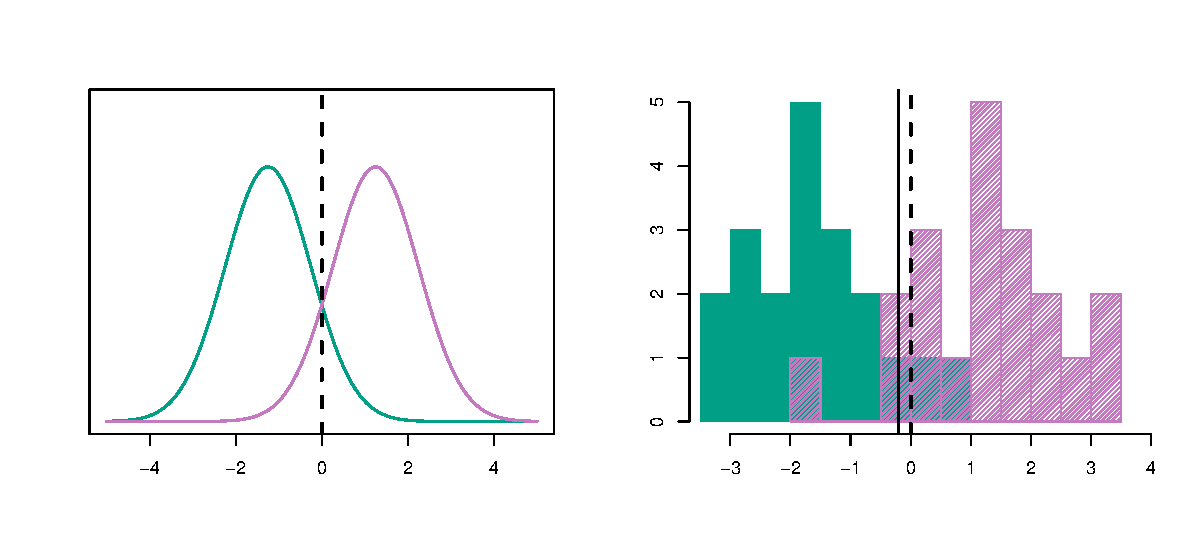
\includegraphics[width=.8\textwidth,trim={280 12mm 10mm 15mm},clip]{4-4}
    \caption{Bayes decision boundary (dashed) and LDA decision boundary (solid) estimated from the training data
      } %: Class 1 (green) and Class 2 (purple).}
  \end{figure}
\end{minipage}\hfill\pause
\begin{minipage}[t]{.49\linewidth}\small
  \textbf{Classes:} Class 1 (green); Class 2 (purple)\\\pause
  \textbf{Sample size and priors:}\pause
  \begin{eqnarray*}
    n_1 &=& n_2 = 20 \\\pause
    \hat\pi_1 &=& \hat\pi_2 = \pause \fr{20}{40} = \pause 0.5 
  \end{eqnarray*}\pause
  \textbf{Decision boundary:}\pause
  \begin{equation*}
    x = \fr{\hat\mu_1 + \hat\mu_2}{2}
  \end{equation*}
  \pause
  \textbf{Performance (error rate):}\\\pause
  Bayes: \pause 10.6\%; \pause
  \note[item]{\rd Question: Is the LDA error rate lower or higher?}
  LDA: \pause 11.1\%
\end{minipage}
\vspace{-2ex}
\end{exampleblock}

\end{frame}

\begin{frame}
  \frametitle{Multiple predictors}
  \pause
  For a {\rd single} predictor $x$, we assumed a \textit{\rd univariate} Gaussian distribution.\pause
  \bigskip

  If we have {\pl multiple predictors}, then:\pause
  \begin{equation}
    \bm x = (x_1, x_2, \ldots, x_D)
  \end{equation}
  \pause
  We then assume sample $\bm x$ has a \textit{\pl multivariate} Gaussian distribution.\pause

      \pgfplotsset{
    colormap={whitered}{color(0cm)=(white); color(1cm)=(purple!75!blue)}
  }
  \begin{figure}[h!]
    \centering
      \begin{tikzpicture}[scale=.4,
    declare function={mu1=1;},
    declare function={mu2=2;},
    declare function={sigma1=0.5;},
    declare function={sigma2=1;},
    declare function={normal(\m,\s)=1/(2*\s*sqrt(pi))*exp(-(x-\m)^2/(2*\s^2));},
    declare function={bivar(\ma,\sa,\mb,\sb)=
      1/(2*pi*\sa*\sb) * exp(-((x-\ma)^2/\sa^2 + (y-\mb)^2/\sb^2))/2;}]
    \begin{axis}[
      colormap name=whitered,
      width=15cm,
      view={45}{65},
      enlargelimits=false,
      grid=major,
      domain=-1:4,
      y domain=-1:4,
      samples=26,
      xlabel={\Large$\bm{x_1}$},
      ylabel={\Large$\bm{x_2}$},
      zlabel={\Large$\bm{p(\bm x)}$},
      colorbar,
      colorbar style={
        at={(1.1,0)},
        anchor=south west,
        height=0.25*\pgfkeysvalueof{/pgfplots/parent axis height},
        title={Density}
      }
      ]
      \only<6->{\addplot3 [surf] {bivar(mu1,sigma1,mu2,sigma2)};}
      \only<7->{\addplot3 [domain=-1:4,samples=31, samples y=0, red, thick, smooth] (x,4,{normal(mu1,sigma1)});}
      \only<8->{\addplot3 [domain=-1:4,samples=31, samples y=0, blue, thick, smooth] (-1,x,{normal(mu2,sigma2)});}

      \only<9->{\draw [black!50] (axis cs:-1,0,0) -- (axis cs:4,0,0);}
      \only<10->{\draw [black!50] (axis cs:0,-1,0) -- (axis cs:0,4,0);}

      \only<11->{\node[blue] at (axis cs:-1,1,0.18) [pin=165:{\Large $f(\bm x_2)$}] {};}
      \only<12->{\node[red] at (axis cs:1.5,4,0.32) [pin=-15:{\Large $f(\bm x_1)$}] {};}
    \end{axis}
  \end{tikzpicture}
  \vspace{-2ex}
    \caption{A multivariate Gaussian density function; $p = 2$ (bivariate Gaussian)}
  \end{figure}
\end{frame}

\begin{frame}
  \frametitle{Multivariate Gaussian distributions: notation }\pause
  If $X$ is a $p$-dimensional normally distributed random variable, then:\pause
  \begin{equation}
    X \sim \mathcal{N}(\mu,\bm\Sigma)
  \end{equation}
  \pause
  where $\mu = \mathbb{E}(\bm x)$ and $\bm\Sigma = Cov(\bm x)$ is the $p\times p$ covariance matrix of $X$.\pause
  \begin{eqnarray}
    Cov(\bm x_j,X_l) &=& \mathbb{E}(\bm x_j - \mathbb{E}(\bm x_j)(\bm x_l  - \mathbb{E}(\bm x_l)) \pause = \mathbb{E}(\bm x_jX_l) - \mathbb{E}(\bm x_j)\mathbb{E}(\bm x_l)\\\pause
     Cov(\bm x_j,X_j) &=& \pause \mathbb{E}(\bm x_j^2) - \lt(\mathbb{E}(\bm x_j)\rt)^2 = \pause \mathbb{V}(\bm x_j)
  \end{eqnarray}
  \pause
  \begin{block}{Probability density function}\pause
    The multivariate Gaussian/normal probability density function (PDF) is given by:\pause
    \begin{equation}
      f(\bm x) = \fr{1}{(2\pi)^{p/2}|\bm\Sigma|^{1/2}}\exp\lt(-\fr12(\bm x-\mu)^T\bm\Sigma^{-1}(\bm x-\mu)\rt)
    \end{equation}
  \end{block}
  
\end{frame}
\begin{frame}
  \frametitle{LDA with multiple predictors}
  \pause
  \begin{itemize}[<+->]
  \item Assume that observations in $c$th class are drawn from multivariate Gaussian $\mathcal{N}({\bm\mu_c},\bm\Sigma)$
    with a common covariance matrix
  \item Estimate distribution parameters $\hat{\bm\mu_c}$, $\hat{\bm\Sigma}$ and priors $\hat\pi_c$:\pause
    \begin{equation}
      \hat{\bm\Sigma} = \fr{1}{n-C}\sum_{c=1}^{C}\sum_{i:y_i = c}(\bm x_i - \hat{\bm\mu_c})(\bm x_i - \hat{\bm\mu_c})^T
    \end{equation}
  \item Compute the linear discriminant functions:\pause
    \begin{equation}\gr 
      \delta_c(\bm x) = x^T\bm\Sigma^{-1}{\bm\mu_c} - \fr12{\bm\mu_c}^T\bm\Sigma^{-1}{\bm\mu_c} + \log\pi_c
    \end{equation}
  \item Assign each observation $x_i$ to the class $c$ which maximizes the linear discriminant functions:\pause
    \begin{equation}
      \hat y_i = \arg\max_c\delta_c(\bm x)
    \end{equation}
\end{itemize}

\end{frame}

\begin{frame}
  \frametitle{LDA with multiple predictors: illustration}
  \pause
  \begin{figure}[h!]
    \centering
    \includegraphics<2->[width=\textwidth]{4-6}
    \caption{LDA for $p=2, C=3$. (L) Conditional class distributions of $X$ (95\% probability ellipses). (R) LDA decision boundaries (solid black) and Bayes decision boundaries (dashed lines).}
  \end{figure}
\end{frame}

 \section{LD derivation}

\begin{frame}
  \frametitle{Bayes' theorem for classification}
  \pause
  Define:
  \begin{align*}
    C      &= \text{number of classes} \\
    \pi_c  &= \text{prior probability that random observation is in $c$th class} \\
    p_c(\bm x) &= \Pr(\bm x = x| Y = c) \quad \text{(conditional probability distribution of $X$)} 
  \end{align*}
  \pause
  According to Bayes' theorem, the \textbf{\bl posterior probability} that an observation is in class $c$ given $x$ is:\pause
  \begin{equation}
    \label{eq:1}\bl
    \Pr(Y=c|X=x) = \fr{\pi_cp_c(\bm x)}{\sum_{l=1}^C\pi_lf_l(\bm x)}
  \end{equation}\pause
  We can also express the posterior probability as:\pause
  \begin{equation}
    \label{eq:2}
    p_c(\bm x) = \Pr(Y=c|X=x) 
  \end{equation}
\end{frame}
\begin{frame}
  \frametitle{Bayes' theorem for classification (cont.)}
  Steps:
  \begin{enumerate}[<+->]
  \item Determine the probability density function of $X$: $p_c(\bm x)$\\[2mm]
  \item Determine the prior probability $\pi_c$\\[2mm]
  \item Compute the posterior probability $p_c(\bm x)$ using Bayes' theorem\\[2mm]
  \item Classify the observation based on the maximum probability:
    \begin{equation}
      \label{eq:3}
      \rd \hat y_i = c^* = \arg\max_c p_c(\bm x_i)
    \end{equation}
    \pause
    Eq.\ \eqref{eq:3} is called the \textbf{\rd decision rule}.
  \end{enumerate}
\end{frame}

\begin{frame}
  \frametitle{Assumptions}
  \begin{block}{Assumption 1}
  $X$ is normally distributed:
  \begin{equation}
    \label{eq:4}
    p_c(\bm x) = \fr{1}{\sqrt{2\pi}\sigma_c}\exp\lt( - \fr1{2\sigma_c^2}(\bm x - {\bm\mu_c})^2\rt)
\end{equation}
where ${\bm\mu_c}$ and $\sigma_c^2$ are the mean and variance of the observations in the $c$th class.
\end{block}
\pause
\begin{block}{Assumption 2}
  There is a common variance across all $C$ classes:\pause
  \begin{equation}
    \label{eq:5}
    \sigma_1^2 = \cdots = \pause \sigma_C^2
  \end{equation}
\end{block}
\end{frame}

\begin{frame}
  \frametitle{Bayes classifier}
  \pause

  Given the assumptions of normally distributed $X$ and constant variance, then the \textbf{\bl posterior probability} according to Bayes is:
  \pause
  \begin{equation}
    \label{eq:6}\bl
    p_c(\bm x) = \fr{\pi_c \fr{1}{\sqrt{2\pi}\sigma_c}\exp\lt( - \fr1{2\sigma_c^2}(\bm x - {\bm\mu_c})^2\rt) }
    {\sum_{l=1}^C \pi_l \fr{1}{\sqrt{2\pi}\sigma_l}\exp\lt( - \fr1{2\sigma_l^2}(\bm x - \mu_l)^2\rt)}
  \end{equation}
  \pause
  The Bayes classifier assigns an observation to the class for which $p_c(\bm x)$ is the largest.\pause
  \bigskip

  For the $i$th observation, this assignment can be written as:\pause
  \begin{equation}
    \label{eq:7}
    y_i = c^* = \arg\max_c p_c(\bm x) = \pause \arg\max_c \log (p_c(\bm x)) = \pause \arg\max_c\delta_c(\bm x)
  \end{equation}

  The term $\gr \delta_c(\bm x) $ denotes the \textbf{\gr linear discriminant functions}.
  \note[item]{The symbol $\arg\max$ means we take the variable that optimizes the objective function instead of the optimal objective value $\max$}.
\end{frame}

\begin{frame}
  \frametitle{Linear discriminant functions}  \pause
  To derive,  take the log of the posterior probability:\pause
  \begin{align*}
    % p_c(\bm x) &= \fr{\pi_c \fr{1}{\sqrt{2\pi\sigma_c}}\exp\lt( - \fr1{2\sigma_c^2}(\bm x - {\bm\mu_c})^2\rt) }
    %          {\sum_{l=1}^C \pi_l \fr{1}{\sqrt{2\pi\sigma_l}}\exp\lt( - \fr1{2\sigma_l^2}(\bm x - \mu_l)^2\rt)}\\
    \log(p_c(\bm x)) &= \log\lt(\fr{\pi_c}{\sqrt{2\pi}\sigma_c}\rt) - \fr{(\bm x - {\bm\mu_c})^2}{2\sigma_c^2}
                   - \sum_{l=1}^C \lt[ \log\lt(\fr{\pi_l}{\sqrt{2\pi}\sigma_l}\rt)  - \fr{(\bm x - \mu_l)^2}{2\sigma_l^2} \rt]\\
      &= \log\lt(\fr{\pi_c}{\sqrt{2\pi}\sigma}\rt) - \fr{(\bm x - {\bm\mu_c})^2}{2\sigma^2}
        - \sum_{l=1}^C \lt[ \log\lt(\fr{\pi_l}{\sqrt{2\pi}\sigma}\rt)  - \fr{(\bm x - \mu_l)^2}{2\sigma^2} \rt]\\
           &= {\gr \log(\pi_c) } {\og \, - \, \log\lt(\sqrt{2\pi}\sigma\rt) - \fr{x^2}{2\sigma^2}}
             {\gr \, + \, \fr{x{\bm\mu_c}}{2\sigma^2} - \fr{{\bm\mu_c}^2}{2\sigma^2}}\\
         &\quad {\og - \sum_{l=1}^C \lt[ \log\lt(\fr{\pi_l}{\sqrt{2\pi}\sigma}\rt)  - \fr{(\bm x - \mu_l)^2}{2\sigma^2} \rt]}
  \end{align*}
  To find the maximizing value of $\log (p_c(\bm x))$, {\og we discard the terms that are constant in $c$} and thus obtain the \textbf{\gr linear discriminant functions}:
  \begin{equation}\gr
    \delta_c(\bm x) =\log(\pi_c) + x\fr{{\bm\mu_c}}{\sigma^2} - \fr{{\bm\mu_c}^2}{2\sigma^2}    
  \end{equation}
  \note[item]{They are called linear discriminant functions because they are linear in $x$}
\end{frame}

\begin{frame}
  \frametitle{Linear discriminant functions (cont.)}\pause
  Given $C$ classes each with priors $\pi_c$, means ${\bm\mu_c}$ and common variance $\sigma$, we express the discrimant function as:\pause
  \begin{align*}
    \delta_1(\bm x) & =\log(\pi_1) + x\fr{\mu_1}{\sigma^2} - \fr{\mu_1^2}{2\sigma^2}\\\pause
    \delta_2(\bm x) & =\log(\pi_2) + x\fr{{\bm\mu_2}}{\sigma^2} - \fr{{\bm\mu_2}^2}{2\sigma^2}\\\pause
    \vdots & \qquad \qquad \vdots  \\\pause
    \delta_C(\bm x) & =\log(\pi_C) + x\fr{{\bm\mu_c}}{\sigma^2} - \fr{{\bm\mu_c}^2}{2\sigma^2}
  \end{align*}
  \pause
  For an observation with $X=x$, the \textit{decision rule} assigns $Y$ to the class $c$ for which $\delta_c(\bm x)$ is the greatest.
\end{frame}

\begin{frame}
  \frametitle{Bayes decision boundary: binary case}\pause
  In the binary case, $C = 2$. \pause The discriminant functions are:\pause
  \begin{align*}
    \delta_1(\bm x) & =\log(\pi_1) + x\fr{\mu_1}{\sigma^2} - \fr{\mu_1^2}{2\sigma^2}\\\pause
    \delta_2(\bm x) & =\log(\pi_2) + x\fr{{\bm\mu_2}}{\sigma^2} - \fr{{\bm\mu_2}^2}{2\sigma^2}
  \end{align*}
  \pause
  The decision rule assigns an observation to Class 1 if $\delta_1(\bm x) > \delta_2(\bm x)$.\pause

  Now, consider the situation where the \textit{\gr priors are equal}:\pause
  \begin{equation*}\gr
    \pi_1 = \pi_2
  \end{equation*}
  \pause
  implying that an observation is \textit{\gr equally likely} to come from Class 1 or Class 2. \pause
  The decision rule would then \textbf{\rd assign to Class 1} if:\pause
  \begin{align*}
     x\fr{\mu_1}{\sigma^2} - \fr{\mu_1^2}{2\sigma^2} &>
              x\fr{{\bm\mu_2}}{\sigma^2} - \fr{{\bm\mu_2}^2}{2\sigma^2}\\\pause
 \implies \rd \quad  x\lt( {\bm\mu_1} - {\bm\mu_2} \rt) & \rd > \fr{{\bm\mu_1}^2 - {\bm\mu_2}^2}{2} %= \pause \fr{({\bm\mu_1}-{\bm\mu_2})({\bm\mu_1}+{\bm\mu_2})}{2} 
%\rd  x &\rd > \fr{({\bm\mu_1}+{\bm\mu_2})}{2}   
  \end{align*}
  \note[item]{Think of the prior as the fraction of observations in a class among all the observations}
  \note[item]{We need to be careful about dividing by $({\bm\mu_1}-{\bm\mu_2})$ because the difference could be negative and thus change the direction of the inequality.}
\end{frame}
\begin{frame}
  \frametitle{Bayes decision boundary (cont.)}
  At the Bayes decision boundary, the $\delta_1 = \delta_2$, thus:\pause
  \begin{align*}
    x\lt( {\bm\mu_1} - {\bm\mu_2} \rt) &= \fr{{\bm\mu_1}^2 - {\bm\mu_2}^2}{2} = \pause \fr{({\bm\mu_1}-{\bm\mu_2})({\bm\mu_1}+{\bm\mu_2})}{2} \\
    x &= \fr{({\bm\mu_1}+{\bm\mu_2})}{2}  
  \end{align*}\pause
  Thus, given a univariate predictor $X$ whose two classes have equal priors $\pi_1 = \pi_2$, the decision boundary lies midway between the means ${\bm\mu_1}$ and ${\bm\mu_2}$.\pause
  \begin{figure}[h!]
    \centering
    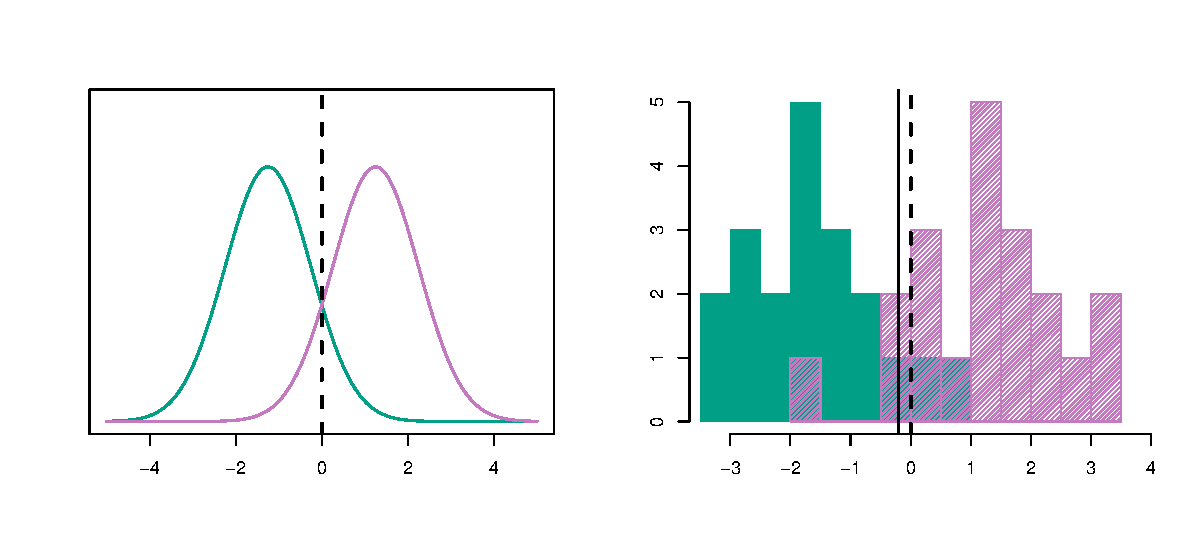
\includegraphics[width=.4\textwidth,trim={0 12mm 100mm 10mm},clip]{4-4}
    \caption{Bayes decision boundary (dashed line) shown for the priors of the distributions of 2 classes: Class 1 (green) and Class 2 (purple)}
  \end{figure}
\end{frame}


\section{QDA}
\begin{frame}
  \frametitle{Quadratic discriminant analysis (QDA)}
  \begin{itemize}[<+->]
  \item A key assumption in LDA is that all classes share a common covariance structure: $\bm\Sigma_1 = \ldots = \bm\Sigma_C = \bm\Sigma$.
  \item If we discard this assumption, then:\pause
    \begin{equation}
      X \sim \mathcal{N}({\bm\mu_c},\bm\Sigma_{\rd c})
    \end{equation}\pause
    and we can no longer ignore the $\hat{\bm\Sigma}_c$ terms in posterior probabilities.
  \item This results in discriminant functions that are \textbf{\gr quadratic} in $x$:\pause
    \begin{eqnarray}
         \delta_c(\bm x) &=& {\gr -\fr12(\bm x-\hat{\bm\mu_c})^T\bm\Sigma_c^{-1}(\bm x-\hat{\bm\mu_c})} - \fr12\log|\bm\Sigma_c|
        + \log\pi_c \\\pause
        &=& {\gr -\fr12x^T\bm\Sigma_c^{-1}\bm x} + x^T\bm\Sigma_c^{-1}{\bm\mu_c} - \fr12\hat{\bm\mu_c}^T\bm\Sigma_c^{-1}\hat{\bm\mu_c}
        - \fr12\log|\bm\Sigma_c| + \log\pi_c
    \end{eqnarray}
  \item Under this assumption of class-specific covariance, we perform \textbf{quadratic discriminant analysis}.
  \end{itemize}
\end{frame}

\begin{frame}
  \frametitle{QDA considerations: bias-variance trade-off}
  \pause
  Number of parameters:\pause
  \begin{itemize}[<+->]
  \item To find $\hat{\bm\Sigma}$ in LDA, $D(D+1)/2$ parameters must be estimated
  \item In QDA, since there are $C$ covariance matrices, $CD(D+1)/2$ must be estimated
  \end{itemize}
  \pause

  \bigskip
  Bias-variance: \pause
  \begin{itemize}[<+->]
  \item Thus QDA is more flexible (lower bias, but potentially higher variance)
  \item LDA might be more stable (lower variance, but potentially higher bias) if the constant $\bm\Sigma$ assumption does not hold for the data.
  \item Generally, with fewer observations, LDA is preferred
  \end{itemize}
\end{frame}

\begin{frame}
  \frametitle{QDA vs. LDA}
  \pause
  QDA produces a quadratic decision boundary which performs better in classifying the observations if the covariance matrices  are different for each class.
  \pause
  
  \begin{figure}[h!]
    \centering
    \includegraphics<3->[width=.9\textwidth]{4-9}
    \caption{(L): shared covariance across classes (linear boundary). (R): different covariance in each class (quadratic boundary). Bayes (purple dashed); LDA (black dotted); QDA (green solid)}
  \end{figure}
\end{frame}

\begin{frame}
  \frametitle{Approximating a quadratic decision boundary}
  \pause
  QDA can be approximated by LDA by including second-order terms in the predictor space, i.e.\pause
  \begin{equation*}
    (X_1,X_2) \to (X_1, X_2, X_1X_2, X_1^2,X_2^2)
  \end{equation*}
  \pause
  The LDA approximation is may be less accurate but more stable, as fewer parameters are required.\pause
  \only<5->{
  \begin{figure}[h!]
    \centering
    \includegraphics<5->[width=.7\textwidth,trim={10mm 130mm 10mm 70mm},clip]{ESL4-6}
    \caption{(L) LDA approximation of decision boundary. (R) QDA decision boundary. $D = 2, C = 3$.}
  \end{figure}}
\end{frame}

\section{Summary}



\begin{frame}
  \frametitle{Outlook}
  \pause
  \begin{itemize}
  \item Next lecture: L2b: Logistic regression\pe
  \item Reading for today's lecture: \pause  \textbf{PMLI} 9.1-2; \textbf{ESL} 4.3\pe
  \item Optional: Naive Bayes classifier (NBC) \textbf{PMLI} 9.3
   \end{itemize}

  

\end{frame}

%\appendix
\appendix\addtocounter{part}{-1}

% \hyperlink{summary-cont}{\beamerbutton{Back}}

\section{Appendix: GLMs}

\begin{frame}
  \frametitle{The generalized linear model (GLM)}
  \label{glm}
  \pause

  \begin{itemize}
  \item Conventional linear models have the form:
    \begin{equation}
      y_{i} \sim N(\bm x_{i}^{T}\bm\beta, \sigma^{2})
    \end{equation}
    \pause where \pause
    \begin{itemize}
    \item $y_{i}$ is a continuous response
    \item $\bm x_{i}$ is a vector of quantitative and/or qualitative explanatory variables
    \end{itemize}
    \pause

  \item Generalized linear models (GLMs) were introduced to extend this framework to allow $y_{i}$ to be modeled by other \href{https://people.eecs.berkeley.edu/~jordan/courses/260-spring10/other-readings/chapter8.pdf}{exponential family distributions} besides the normal/Gaussian, e.g.
    \begin{itemize}
    \item exponential
    \item binomial/multinomial (with fixed number of trials)
    \item Poisson
    \end{itemize}
  \pause

\item In the GLM framework: \pause
  \begin{itemize}
  \item The mean of $y_{i}$ is given by $\mu_{i}$
  \item $\mu_{i}$ can be specified by a nonlinear function of $\bm x_{i}^{T}\bm\beta$
  \item Note that the simple linear regression is a special case of GLM in which $\mu_{i} = \bm x_{i}^{T}\bm\beta$ and $y_{i}$ follows a Gaussian distribution
  \end{itemize}
    \end{itemize}

    \pause

    \hyperlink{recap}{\beamerbutton{Back to Recap}}
  \end{frame}

  \begin{frame}
    \frametitle{GLM components}

    \pause

    A GLM consists of three parts: \pause

    \begin{itemize}
    \item \textbf{Random component:} this is the probability distribution of the response variable \pause
    \item \textbf{Systematic component:} specifies the explanatory variables within the linear combination of their coefficients ($\bm X\bm\beta$)\pause
    \item \textbf{Link function $\bm{g(\mu)}$:} defines the relationship between the random and systematic components: \pause
      \begin{itemize}
      \item Simple linear regression (identity link function): \pause
        \begin{equation}
          g(\mu_{i}) = g(\mathbb{E}(y_{i})) = \bm x_{i}^{T}\bm\beta
        \end{equation}
        \pause
      \item Binary logistic regression (logit link function): \pause
        \begin{equation}
          g(\mu_{i}) = g(p(\bm x_{i})) = \pause \text{logit} (p(\bm x_{i})) = \pause
          \ln\lt(\fr{p(\bm x_{i})}{1 - p(\bm x_{i})} \rt) = \pause \bm x_{i}^{T}\bm\beta
        \end{equation}
      \end{itemize}
    \end{itemize}
  \end{frame}

  \begin{frame}
    \frametitle{Assumptions of GLM}
    \pause
    \begin{itemize}
    \item The observations of the response variable $\bm y$  are i.i.d.
      \pause
    \item Response variable $y_{i}$ is typically exponentially distributed (not restricted to being normally distributed) \pause
      \begin{itemize}
      \item Implies that errors need not be normally distributed (but should be independent)
      \end{itemize}
    \item Link function is linear with respect to the coefficients ($\beta_{j}$)\pause
      \begin{itemize}
      \item Relationship between response and explanatory variables does not have to be linear \pause
      \item Explanatory variables can be nonlinear transformations of original values (as in simple linear regression)
      \end{itemize}
      \pause
    \item Variance may not homogeneous (i.e.\ homoscedasticity is not a requirement)\pause
    \item Parameters are estimated via MLE 
    \end{itemize}
  \end{frame}

  \begin{frame}
    \frametitle{Commonly used GLM models and their components}

    \pause

    \begin{center}\small
      \begin{tabular}{l p{.7in} l }\toprule
        \bf Model & \bf Random component& \bf Link function   \\\midrule
        Linear regression & Gaussian & Identity: $g(\mu_i) = \mu_{i} = \beta^{T}x_{i}$ \\\midrule
        Binary logistic regression & Bernoulli & Logit:  $g(\mu_{i}) = \ln\lt(\fr{\mu_{i}}{1 - \mu_{i}}\rt)$ \\\midrule
        Probit regression & Bernoulli & Probit: $g(\mu_{i}) = \Phi^{-1}(\mu_{i})$ \\\midrule
        Multinomial logit/logistic  & Categorical & Multinomial logit: $g(\mu_{ic}) = \ln\lt(\fr{\mu_{ic}}{\mu_{iC}}\rt)$ \\\midrule
        Poisson regression & Poisson & Log: $g(\mu_{i}) = \ln(\mu_{i})$ \\\bottomrule
      \end{tabular}
    \end{center}

    \pause

    Note that in all cases, the link function always results in:
    \begin{equation}
      g(\mu_i) = \beta^{T}x_{i}
    \end{equation}
    \pause Its job is to ``link'' the response to the systematic component via a suitable transformation that results in a linear function of the $\beta$'s.
  \end{frame}

  \begin{frame}
    \frametitle{Further reading on GLMs}
    \pause

    \begin{itemize}
    \item German Rodriguez's lecture notes on GLMs: \url{https://data.princeton.edu/wws509/notes/}
    \item Penn State: \url{https://online.stat.psu.edu/stat504/lesson/6/6.1} (Including more on logistic and multinomial logistic)
    \end{itemize}
  \end{frame}

 
\end{document}

%%% Local Variables:
%%% mode: latex
%%% TeX-master: t
%%% End:
